\section{Features}
The Mobility Features were implemented according to the definitions given in \ref{chapter:03-design}

\section{Tuning Parameters}
Parameter tuning was done by taking a few different examples where ground truth is  known, i.e. by having done it myself. The examples include whole days in Munich (GER), Copenhagen (DK) and Bornholm (DK) which all have vastly different environments and acitivties, with Munich having places displaced very far away and where public transportation was necessary. In Copenhagen I travelled by foot, either walking or running and on Bornholm I would travel in the city of Rønne by foot, again walking or running, or going to the other side of the island by car, and walking the dog. Since the ground truth is known for each of these examples, the parameter tuning is done by taking the parameters with the biggest impact such as stop duration and place radius, starting high and then lowering the parameter value until a reasonable result is achieved across the board.


\subsubsection{Number of Clusters}
Defined as the number of non-negative place labels found by the Places algorithm.

\begin{minted}{python}
def num_clusters(places):
    return len(places > 0)
\end{minted}

\subsubsection{Location Variance (LV)} 
LV was computed as the natural logarithm of the sum of the statistical variances of the latitude and the longitude components of the location data. The dataset must contain at least 2 observations to calculate the variance, otherwise the variance of both the latitude- and the longitude will be zero, and thus $LV = log(0 + 0 + 1)  = 0$

\begin{minted}{python}
def location_variance(dataset):
    return log(var(dataset.lat) + var(dataset.lon.var) + 1)
\end{minted}

\subsubsection{Location Entropy (LE)} 
Here, we use the duration spent at each place, found in the duration column in the places dataframe.

\begin{minted}{python}
def entropy(places):
    p = places.duration / sum(places.duration)
    return -sum(p * log(p))
\end{minted}

\subsubsection{Normalized LE} 
Here we just divide LE by the log to the number of places.

\begin{minted}{python}
def normalized_entropy(places):
    return entropy(places) / log(places.length)
\end{minted}

\subsubsection{Time-distribution Table}
The time distribution table tells the story of which places were visited for how long during the day and does this by dividing the day into 24 one-hour time slots represented by rows, and the columns representing the different significant places found by the pre-processing algorithms. Each entry $T[i,j]$ is the number of hours spent at timeslot $i$ at place $j$, which means that the row can maximally sum to 1.0. If the user moves between two places, the row will however not sum to 1.0 since there was time spent at none of the places.

Using the stops, the time spent at each place can be calculated for each hourly timeslot during the day. Concretely, this is done by iterating through each stop and incrementing the time at entry $i,j$ using the arrival time of the stop \verb|1 - row.arrival.minute / 60| by using the \verb|arrival.hour| as the hour slot. For the last time slot the same is done, but using the departure time \verb|row.departure.minute / 60|. Every time slot in between for the the place $j$ is set to 1.0 since the user was there for the full time slot.

\begin{minted}{python}
def make_hour_matrix(stops, num_places):
    h = np.zeros((HOURS_IN_A_DAY, num_places))
    
    for index, row in stops.iterrows():
        pid = row.place
        start_hour = row.arrival.hour
        end_hour   = row.departure.hour
        
        # If user arrived and departed within the same hour
        # Then the time stayed is the diff between departure and arrival
        if start_hour == end_hour:
            h[start_hour, pid] = row.departure.minute - row.arrival.minute
        
        else:
            # Arrival hour
            h[start_hour, pid] = 60 - row.arrival.minute

            # In between
            for hour in range(start_hour+1, end_hour):
                h[hour, pid] = 60

            # Departure hour
            h[end_hour, pid] = row.departure.minute
        
    return h / 60 # Normalize by 60 mins
\end{minted}



\subsubsection{Home Stay} 
The percentage of time the participant has been home place, home being the most visited cluster between 12 am and 6 am which can be identified by using the mean of the the historical time distribution tables, i.e. the place which, on average, was the most visited between 00 and 06 am. Afterwards, all the stops during the day are iterated and the duration of the stops belonging to the home cluster are summed up.

\subsubsection{Transition Time} 
To calculate the transition time of the user the Moves are used, and the difference is time stamps between all the individual data points which make up each move are summed together. 

\subsubsection{Total Distance} 
Same procedure as transition time, except for using the the distances between all the individual data points rather than the duration.


\begin{figure}
    \centering
    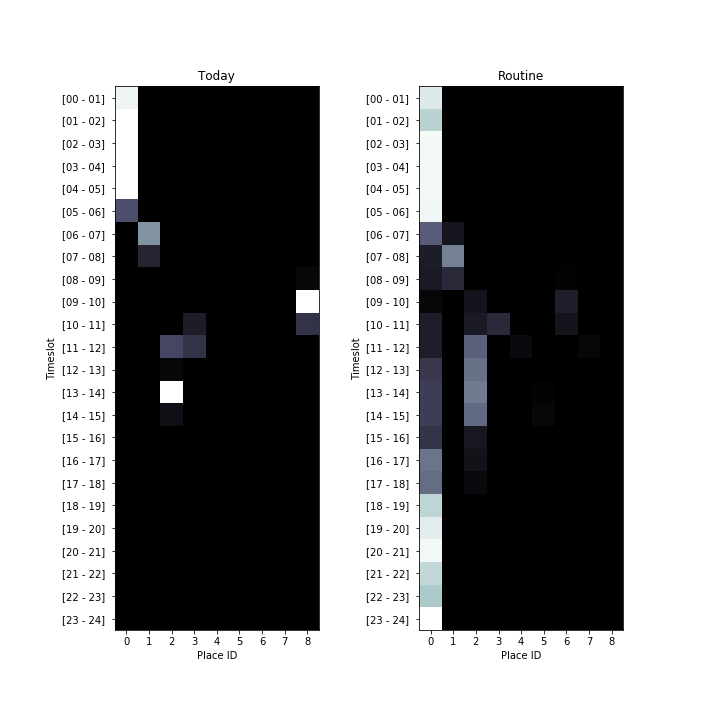
\includegraphics[width=\textwidth]{images/routine.png}
    \caption{An hour matrix of a specific day compared to the Routine Matrix derived from several days of data.}
    \label{fig:routine_example}
\end{figure}


